\section{K4 - BKR.kr - 1 - Radfahrer - OA - MK}

\begin{langesbeispiel} \item[1] %PUNKTE DES BEISPIELS
Zwei Radfahrer fahren in entgegengesetzter Richtung durch eine Kurve. Welchen Weg legt jeder von ihnen zurück, wenn sie jeweils am äußersten rechten Fahrbahnrand fahren? (Runde auf 2 Dezimalstellen)
				\begin{center}
					\resizebox{0.4\linewidth}{!}{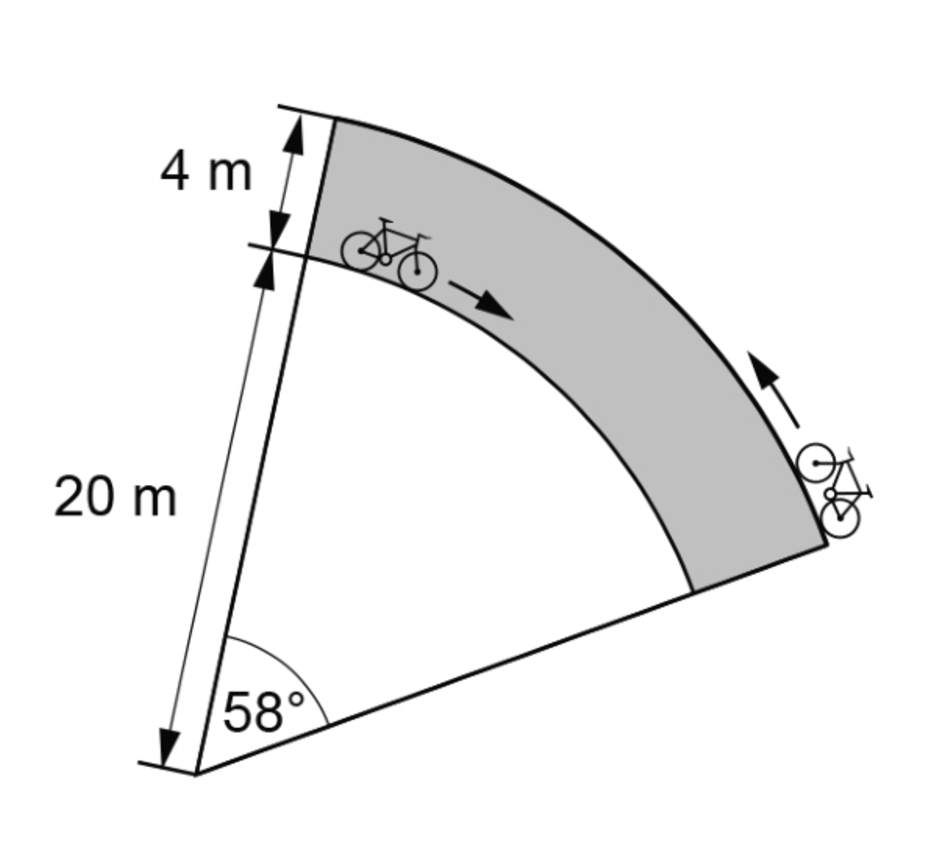
\includegraphics{../_database/Bilder/K4_1_radfahrer.eps}}
				\end{center}
				
				\antwort{Fahrrad 1:
				
				$b=\frac{r\cdot\pi\cdot\alpha}{180}=\frac{20\cdot\pi\cdot 58}{180}=20,25$
				
				Fahrrad 2:
				
				$b=\frac{r\cdot\pi\cdot\alpha}{180}=\frac{24\cdot\pi\cdot 58}{180}=24,3$}
\end{langesbeispiel}